%
% Unless otherwise indicated, the copyright in this material is 
% owned by Joerg Evermann. This material is licensed to you under the 
% Creative Commons by-attribution non-commercial license (CC BY-NC 4.0)}
%
\section*{Learning Goals}

After reading this chapter, you should be able to:
\begin{itemize}
   \item Explain and calculate basic one-dimensional and two-dimensional convolutions, including padding and striding.
   \item Explain the purpose of different pooling methods for convolutional networks and calculate basic pooling in one and two dimensions.
   \item Explain the building blocks of a ConvNet for classification, their purpose, and the concept of a feature map.
   \item  Build convolutional networks for image and text classification using popular neural network software tools.
   \item Explain the concept of a word embedding and its use in neural networks.
\end{itemize}

\section*{Sources and Further Reading}

The material in this chapter is based on the following sources. 

\begin{resourcebox}
Kevin P. Murphy: \emph{Probabilistic Machine Learning -- An Introduction}. MIT Press 2022. \\

\small\url{https://probml.github.io/pml-book/book1.html}\normalsize \\

Chapter 13, 14, 15
\end{resourcebox}

The book by Murphy is freely available and provides three chapters on neural networks, one for structured data, one for images, and one for sequences. It provides significant depth on convolutional and recurrent network architectures, fitting the models, and problems that the data analyst may encounter. 

\begin{resourcebox}
Tensorflow Guides: \\

\small\url{https://www.tensorflow.org/guide}\normalsize \\

\small\url{https://www.tensorflow.org/tutorials/load_data/text}\normalsize
\end{resourcebox}

This course uses the Tensorflow programming framework for neural network applications. The Tensorflow website has a multitude of introductory and advanced guides and tutorial that cover all aspects of machine learning with neural networks. 

\section{Introduction}

Convolutional Neural Networks (CNNs) are a class of deep neural networks, most commonly applied to analyzing images. They are also known as \emph{ConvNets} and are particularly powerful for tasks like image recognition and classification. CNNs have been successful in identifying faces, objects, and traffic signs as well as powering vision in robots and self driving cars. CNNs as they are known today were popularized in the 1990s by Yann LeCun and his colleagues, who used them for digit recognition in postal codes. 

The primary motivation for convolutional networks stems from the limitations of fully connected networks in image processing. Fully connected networks that treat input pixels independently lack the spatial hierarchies of features in an image, which leads to inefficiencies and a loss of spatial relationships among pixels. CNNs address these issues by leveraging spatial hierarchies through localized receptive fields called \emph{convolution filters}, shared weights, and pooling, which results in robustness to image transformations and significant reduction in the number of parameters needed.

At its core, a CNN automatically learns and identifies various features in images at multiple levels of abstraction. For example, the initial layers might detect edges and textures, intermediate layers learn to identify larger motifs, and deeper layers interpret these motifs as parts of familiar objects. CNNs have been successfully applied in a wide range of visual data applications, including:

\begin{itemize}
\item \emph{Image and Video Recognition:} CNNs can classify images and videos into categories, often surpassing human performance in tasks such as facial recognition and object detection.
\item \emph{Medical Image Analysis:} In healthcare, CNNs are used for diagnosing diseases by analyzing medical scans to detect anomalies like tumors in MRI scans or X-rays.
\item \emph{Autonomous Vehicles:} They help in identifying obstacles, understanding traffic signs, and enabling vehicles to make informed decisions.
\item \emph{Augmented Reality:} CNNs can augment real-world environments by enhancing image and video feeds in real-time, providing a richer user experience.
\end{itemize}

CNNs represent a significant advancement in the ability to automatically interpret large sets of visual data, leading to improvements across various applications that require automatic visual recognition. Their ability to understand the complexity of images and videos with increasing accuracy has made them the backbone of modern artificial intelligence in the visual domain.

\section{Convolutional Layers}

A \emph{convolutional layer}\index{Convolutional layer} is a fundamental building block of a Convolutional Neural Network (ConvNet)\index{Convolutional neural network}\index{ConvNet|see{Convolutional neural network}}. It performs the primary operations that allow a ConvNet to capitalize on the spatial structure of input data, such as images, by extracting features that become increasingly complex and high-level as data progresses through deeper layers of the network.

A convolutional layer applies a set of learnable \emph{convolution filters} (also known as \emph{convolution kernels})\index{Convolution filter}\index{Convolution kernel|see{Convolutional filter}} to the input. Each filter is small spatially (along width and height), but extends through the full depth of the input volume.

The convolution operation involves sliding each filter across the width and height of the input image and computing dot products between the filter and the local regions of the input image. As the filter slides over the input image, a 2-dimensional activation map (or feature map)\index{Feature map}\index{Activation map|see{Feature map}} is created as output that gives the responses of that filter at every spatial position. Intuitively, the network learns filters that activate when they see some specific type of feature at some spatial position in the input.

Figure~\ref{fig:screen1_chap16} shows an example in one dimension. The kernel vector $[1, 2]$ is first multiplied element-wise with the first two elements of the input, yielding $[0,1] \dot [1, 2] = [0, 2]$. The result is then summed, yielding $2$. This is the first element of the output. The kernel is then moved one position to the right. Multiplication with that input portion yields $[1, 2] \dot [1, 2] = [1, 4]$ and summing yields $5$, the second element of the output or activation/feature map. This is done until the kernel is multiplied with the two right-most elements of the input in Figure~\ref{fig:screen1_chap16}. Note that the kernel of length 2 can be applied 6 times to the input of length 7 in Figure~\ref{fig:screen1_chap16}, yielding an output of length 6.

\begin{figure}[b]
\centering
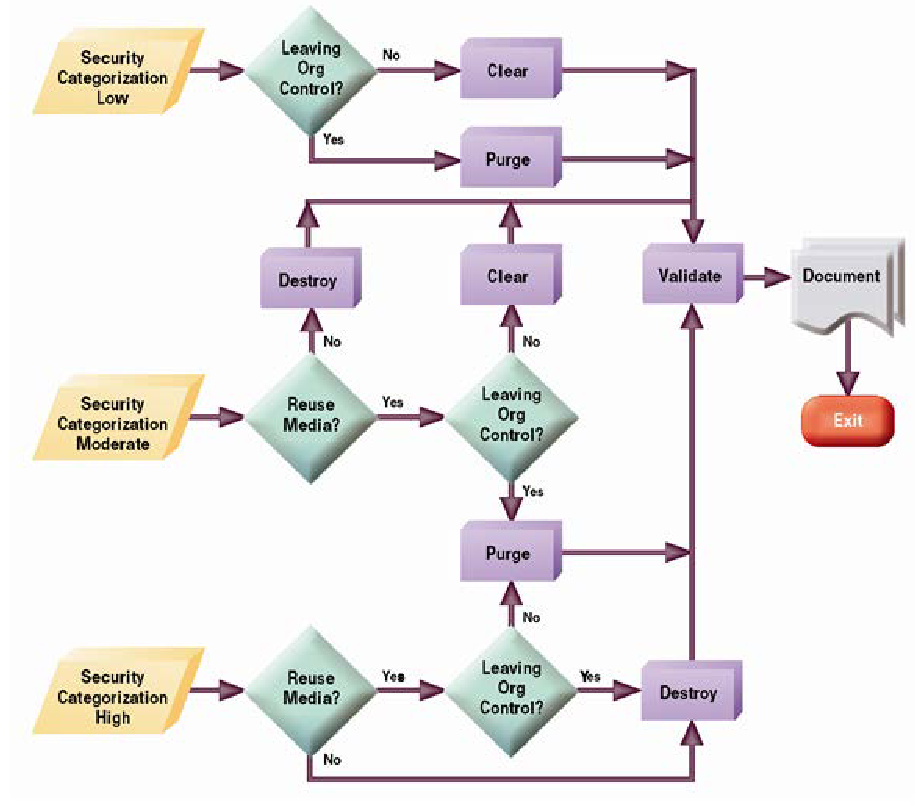
\includegraphics[width=.8\textwidth]{screen1.png} \\

\scriptsize Source: Murphy Fig. 14.4 \normalsize
\caption{1-dimensional convolution filter}
\label{fig:screen1_chap16}
\end{figure}

Figure~\ref{fig:screen2_chap16} shows an example in two dimensions. Here, the first multiplication and summing yields $0 \dot 0 + 1 \dot 1 + 3 \dot 2 + 4 \dot 3 = 19$, which is the top left element of the output in Figure~\ref{fig:screen2_chap16}. The kernel can then be moved once to the right, and once to the bottom. This yields an output shape of $2 \times 2$. 

\begin{figure}
\centering
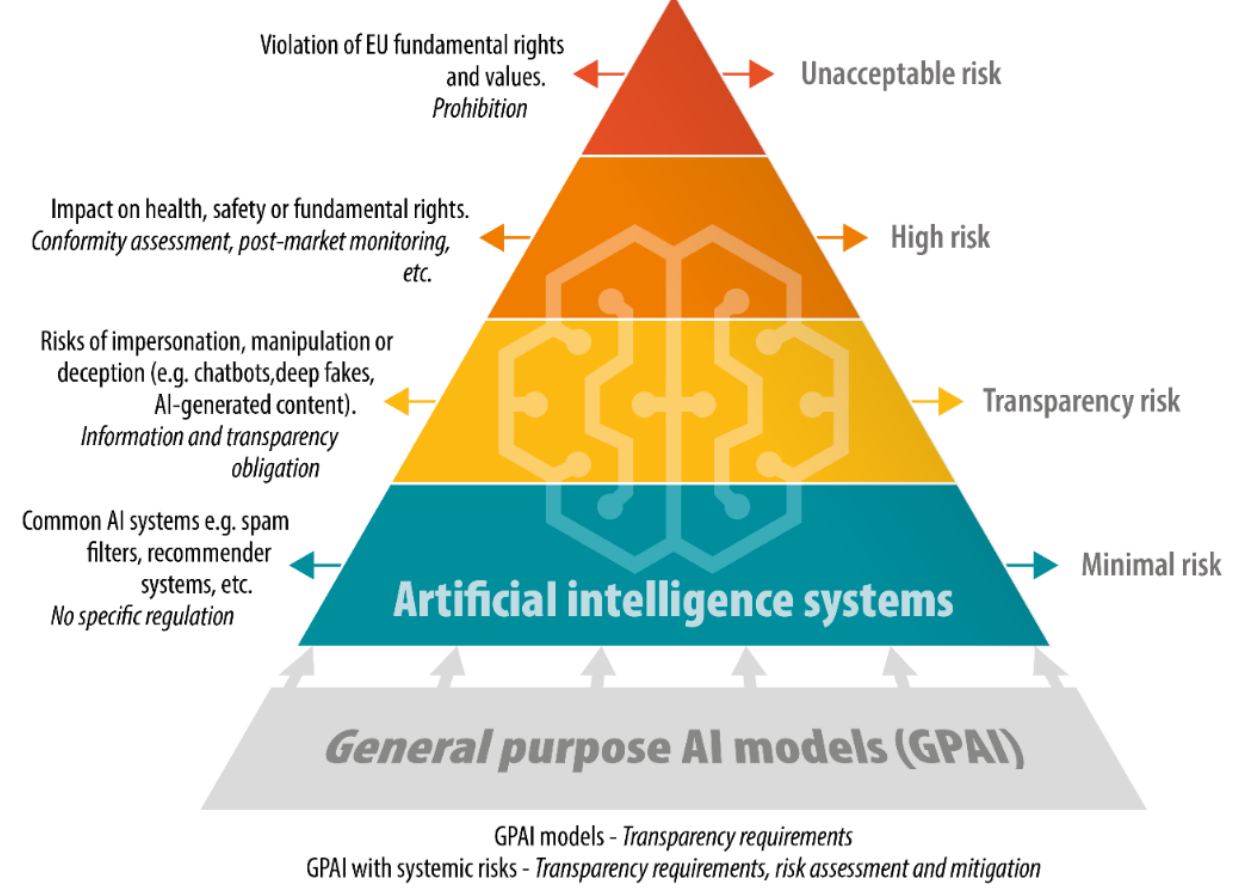
\includegraphics[width=.5\textwidth]{screen2.png} \\

\scriptsize Source: Murphy Fig. 14.5
\caption{2-dimensional convolution filter}
\label{fig:screen2_chap16}
\end{figure}

Figure~\ref{fig:screen3} shows a mulit-channel 2D convolution. The kernel consists of two channels that are applied to two channels of the input. There are as many channels in the kernel as there channels in the input\index{Channel (convolution filter)}. The two channels are then summed to product a single output channel. As a realistic example, consider an RGB image with three ''depth'' channels, one each for the red, green, and blue color components. A kernel might then have a size of $3\times 3 \times 3$ (3 width, 3 height, and 3 for the three color channels).

\begin{figure}[b]
\centering
\includegraphics[width=.8\textwidth]{screen3.png} \\

\scriptsize Source: Murphy Fig. 14.9
\caption{Multi-channel 2D convolution}
\label{fig:screen3}
\end{figure}

A single convolutional network layer may have \emph{multiple filters}. Each filter will yield one output channel or activation/feature map. These output channels are in addition to the depth of each filter. For example, the $2 \times 2 \times 2$ filter applied to the $3 \times 3 \times 2$ input in Figure~\ref{fig:screen3} yielded a single output channel of shape $2 \times 2$. Applying 10 independent filters that are each of shape $2 \times 2 \times 2$ to the input yields an output of shape $2 \times 2 \times 10$.

Consider another simple example in image processing, with an input image of size $32 \times 32 \times 3$ (width x height x channel (red, green, blue)). A convolutional layer might have 10 filters of size $5 \times 5 \times 3$. The output of applying these filters will result in an output of size $28 \times 28 \times 10$ (when using a stride of 1 and no padding, see below).

\begin{alertbox}
While the examples show fixed numbers in the kernels, the kernel elements are actually trainable parameters.
\end{alertbox}

\begin{alertbox}
Verifying the shape/dimensions of inputs, kernels, and outputs, and understanding how they are related to each other is important to understand and to verify the correctness of the implemented model!
\end{alertbox}

There are two key considerations when defining a convolutional network layer, \emph{stride}\index{Striding (in convolutional network)} and \emph{padding}\index{Padding (in convolutional layer)}. When moving the kernel over the input, the \emph{stride} controls the size of the steps in each direction. A stride of $1$ means the kernel moves one column or row at a time. A larger stride results in downsizing of the feature map, in removing redundancy in the output feature map (it avoids an input element being processed multiple times by a filter) and in increasing the efficiency of the data representation in the neural network.

Second, the input is often \emph{padded} with zeros around the edges (''zero-padding''). This allows control over the shape of the output feature map and it also increases the weight or emphasis given to edge values, which are otherwise captured only once by a filter, in contrast to interior values, which are captured multiple times as the kernel moves over the input. Inputs may be padded by one ''frame'' of zeros or by multiple zero-frames, limited only by the size of the convolution kernel.

Figure~\ref{fig:screen4_chap16} shows an example of a zero padded input (bottom, dark gray squares surrounding the light gray squares indicate padding) and a striding of $2$ in each direction. The output feature map is shown on top.  

\begin{figure}
\centering
\includegraphics[width=.66\textwidth]{screen4.png} \\

\scriptsize Source: Murphy Fig. 14.8(b)
\caption{Striding and padding in a convolutional network}
\label{fig:screen4_chap16}
\end{figure}

While the convolution layer may look complicated and complex, it essentially produces a weighted sum of inputs where the convolution kernel entries are the weights, very much like the general neural network unit definition in the previous chapter. A bias term is added to the weighted sum produced by the convolution, before the sum is transformed using a non-linear activation function. In many ConvNets, the activation function is the ReLU (Rectified Linear Unit). In other words, the CNN functions very much like the general neural networks introduced in the previous chapter, except that the connections between inputs and weights are more complex and focus on spatial relationships. As with fully connected networks, it is important to understand the number of parameters (weights and biases) in order to verify the correctness of the implemented model.

As with general neural networks, it is instructive to examine and verify the number of parameters for each CNN layer. Let the kernel be of size $k \times l$ and let the input have $m$ channels. Then, there are $k \times l$ elements for each of the $m$ input dimensions, i.e. a total of $m \times k \times l$ parameters. A CNN layer may produce $n$ different output channels, requiring such a kernel of size $m \times k \times l$ for each of the $n$ output channels, for a total of $n \times m \times k \times l$ parameters. Additionally, there will be one bias term for each of the $n$ output channels, for a total of $n \times m \times k \times l + n$ trainable parameters. \\

\textbf{Example}: Let the kernel size be $5 \times 5$ applied to an input with $3$ channels and an output of $32$ channels. Then, the CNN layer has $32 \times 3 \times 5 \times 5 + 32 = 2432$ parameters.


\begin{exercisebox}

Calculate the number of trainable parameters for the following CNN layers:
\begin{enumerate}
\item A kernel of size $4 \times 4$ operating on an input with 3 channels and an output of 8 channels.
\item A kernel of size $2 \times 2$ operating on an input with 8 channels and an output of 16 channels.
\item A kernel of size $3 \times 3$ operating on an input with 16 channels and an output of 4 channels.
\item A kernel of size $5 \times 5$ operating on an input with 4 channels and an output with 4 channels.
\end{enumerate}
Assume the previous four layers are part of the same neural network, what is the total number of trainable parameters?
\end{exercisebox}



\section{Pooling Layers}

Pooling layers\index{Pooling layer (in convolutional network)} within ConvNets are used to reduce the spatial dimensions (width and height) of the convolution output for the next convolutional layers or for subsequent dense, fully-connected layers. This reduction in dimensions serves several purposes. It decreases the computational load and the memory usage, helps prevent overfitting by providing an abstracted form of the representation, and makes the network invariant to small transformations, distortions, and translations in the input. Pooling is applied separately to each output channel of a convolution. Note that pooling layers do not have trainable parameters.

The most common types of pooling include \emph{max pooling} and \emph{average pooling}. Max pooling partitions the convolution output into a set of overlapping or non-overlapping regions, and outputs the maximum value for each such region. For instance, a $2 \times 2$ max-pooling layer applied with a stride of 2 reduces the size of the input by a factor of four (halving the height and width separately). Instead of taking the maximum value from each distinct region, average pooling computes the average of the values in each patch on a feature map. 

Figure~\ref{fig:screen5_chap16} shows an example of $2 \times 2$ max pooling on a $3 \times 3$ input with stride 1. In this example, the pooling stride is less than the pooling filter size, so that the pooled regions are overlapping. Each convolution output may be captured multiple times in different pooling outputs. When the stride is chosen to the same size as the pooling filter, the regions are not overlapping. Overlapping regions retain more information but are computationally more intensive and require additional memory, as the size of the pooling output and therefore the size of all subsequent layers is larger. 

\begin{figure}
\centering
\includegraphics[width=.5\textwidth]{screen5.png} \\

\scriptsize Source: Murphy Fig. 14.12
\caption{Pooling in a ConvNet}
\label{fig:screen5_chap16}
\end{figure}

In image processing in particular, pooling helps the network become invariant to small translations, rotations, and scalings of an image. Max pooling in particular helps in detecting features like edges, textures, and shapes, even if they appear in different areas of the image in different instances. Although pooling reduces the resolution of the feature map, important features (like the presence of certain edges or textures) are retained due to the nature of max or average operations within localized regions of the input.

\begin{exercisebox}

\begin{enumerate}
\item Assume the following $5 \times 5$ input matrix:
\begin{align*}
\begin{bmatrix} 1 & 2 & 3 & 2 & 1 \\ 
                2 & 3 & 2 & 1 & 3 \\ 
                3 & 2 & 1 & 3 & 2 \\
                2 & 1 & 3 & 2 & 1 \\               
                1 & 3 & 2 & 1 & 3 
\end{bmatrix}
\end{align*}
and the following $3 \times 3$ convolution kernel:
\begin{align*}
\begin{bmatrix}  1 & 2 & 1 \\ 
                2 & 4 & 2 \\
                1 & 2 & 1 \end{bmatrix}
\end{align*}
Zero-pad the matrix with \emph{two} zeros on all sides and using stride 2, calculate the convolution result. What are the dimensions of the convolution output?

\item Apply a $2 \times 2$ max pooling layer to the result of the previous exercise. 
\end{enumerate}
\end{exercisebox}


\section{Understanding ConvNets}

The convolutional and pooling layers of a CNN are only part of the complete neural network. The purpose of the these layers is essentially \emph{feature extraction} or \emph{feature learning}, that is, to identify or learn features in the input that might be useful for subsequent tasks like classification. For images processing tasks, the convolutional and pooling layers may detect features such as edges, textures, geometric shapes, etc. These features are useful in classifying the image content, e.g. does the image show a bee or a tiger. 

Figure~\ref{fig:screen6} shows an example of a complete network. Multiple convolutional and pooling layers are stacked in a sequential model. The output of the final pooling layer is then ''flattened'', that is, the information in the two or three dimensional output (width x height x channels) is arranged linearly in a one-dimensional vector. This vector forms the input to a classification network, which typically consists of a sequence of dense, fully-connected layers and a final softmax output layer, as illustrated in the previous chapter. Thus, one can think of the convolutional part of the network as the feature extraction or feature learning part whose output are the features for the classification part of the network.

\begin{figure}
\centering
\includegraphics[width=\textwidth]{screen6.png} \\

\scriptsize Source: Murphy Fig. 14.13
\caption{Convolutional network for image classification}
\label{fig:screen6}
\end{figure}

Figure~\ref{fig:screen12} shows another useful diagram. In addition to the general architecture it shows the dimensionality of the output at each stage, which is very helpful in understanding how convolution and pooling filters operate. For example, the input image is of shape $224 \times 224 \times 3$. There are 96 convolutional filters operating on this image, each with a kernel shape of $7 \times 7 \times 3$ and a stride of 2. This yields an output with shape $110 \times 110 \times 96$. The subsequent $3 \times 3$ pooling with stride 2 reduces this to $55 \times 55 \times 96$ for the final layer 1 output. 

\begin{alertbox}
Verifying the shape/dimensions of inputs, kernels, and outputs, and understanding how they are related to each other is important to understand and to verify the correctness of the implemented model!
\end{alertbox}

\begin{figure}
\centering
\includegraphics[width=\textwidth]{screen12.png}  \\
\vspace{\baselineskip}

\hrule

\vspace{\baselineskip}
\scriptsize Source: Matthew D. Zeiler and Rob Fergus (2013) Visualizing and Understanding Convolutional Networks. \url{https://doi.org/10.48550/arXiv.1311.2901}

\caption{Convolutional network for image classification, with dimensionality}
\label{fig:screen12}
\end{figure}


\begin{infobox}
This term ''feature map''\index{Feature map} may be used in various ways. Some authors use it to describe the convolution output before the application of activation function and pooling, some authors use it to describe the convolution output after application of the activation function but prior to pooling, some authors use it to describe the output after pooling and some authors use it to describe any of the three. Hence, when the term ''feature map'' is used, it is important to identify the precise meaning in a particular context.
\end{infobox}

To understand how convolutional networks perform feature extraction or feature learning, it is instructive to visualize the feature maps. There are multiple ways of doing this. One of the earliest techniques developed for this is the ''\emph{DeconvNet}\footnote{Matthew D. Zeiler and Rob Fergus (2013) Visualizing and Understanding Convolutional Networks. \url{https://doi.org/10.48550/arXiv.1311.2901}}''. The general architecture of a DeconvNet is shown in Figure~\ref{fig:screen13}. Using an unpooling operation, a DeconvNet successively reconstructs the image input for a feature map\index{DeconvNet}. 

\begin{figure}
\centering
\includegraphics[width=.66\textwidth]{screen13.png} \\

\vspace{\baselineskip}
\scriptsize Source: Matthew D. Zeiler and Rob Fergus (2013) Visualizing and Understanding Convolutional Networks. \url{https://doi.org/10.48550/arXiv.1311.2901}
\caption{DeconvNet architecture}
\label{fig:screen13}
\end{figure}

Figures~\ref{fig:layer1} to \ref{fig:layer45} show reconstructed visualizations for a selection of feature maps in a 5-layer convolutional network. The feature maps on the left of each image give an indication of the type of feature they represent, and the corresponding visualization on the right of each figure gives examples of input images that correspond to the detected features. The images on the right of each figure are not training images, they are reconstructed by the DeconvNet.

\begin{figure}
\centering
\includegraphics[height=2in]{layer1.png} \\
\vspace{\baselineskip}
\scriptsize Source: Matthew D. Zeiler and Rob Fergus (2013) Visualizing and Understanding Convolutional Networks. \url{https://doi.org/10.48550/arXiv.1311.2901}
\caption{Layer 1 feature map visualization by a DeconvNet}
\label{fig:layer1}
\end{figure}

Figure~\ref{fig:layer1} indicates that the first layer appears to have learned to recognize basic features such as edges or image contrasts as well as colours of an image. 

\begin{figure}
\centering
\includegraphics[height=2in]{layer2.png} \\
\vspace{\baselineskip}
\scriptsize Source: Matthew D. Zeiler and Rob Fergus (2013) Visualizing and Understanding Convolutional Networks. \url{https://doi.org/10.48550/arXiv.1311.2901}
\caption{Layer 2 feature map visualization by a DeconvNet}
\label{fig:layer2}
\end{figure}

The second layer in Figure~\ref{fig:layer2} appears to have learned to recognize geometric shapes such as lines, circles, squares, but also colors.

\begin{figure}
\centering
\includegraphics[width=\textwidth]{layer3.png} \\
\vspace{\baselineskip}
\scriptsize Source: Matthew D. Zeiler and Rob Fergus (2013) Visualizing and Understanding Convolutional Networks. \url{https://doi.org/10.48550/arXiv.1311.2901}
\caption{Layer 3 feature map visualization by a DeconvNet}
\label{fig:layer3}
\end{figure}

Layer 3, shown in Figure~\ref{fig:layer3}, has learned to recognize more complex features that resemble simple objects, such as wheels, fruits, people, but also complex geometric patterns. 

\begin{figure}
\centering
\includegraphics[width=\textwidth]{layers45.png} \\
\vspace{0.5\baselineskip}
\scriptsize Source: Matthew D. Zeiler and Rob Fergus (2013) Visualizing and Understanding Convolutional Networks. \url{https://doi.org/10.48550/arXiv.1311.2901}
\caption{Layers 4 and 5 feature map visualization by a DeconvNet}
\label{fig:layer45}
\end{figure}

Finally, layers 4 and 5 have learned to extract specific objects or object parts, such as dogs, birds, but also geometric shapes. The final layer shows a clear ability to extract the presence of specific object classes in an image. 

\FloatBarrier

\section{Image Classification Example using Tensorflow}

This section illustrates how to implement convolutional neural networks in Tensorflow/Keras\footnote{Python code for this example is taken from \href{https://www.tensorflow.org/tutorials/images/cnn}{TensorFlow.org} that is made available under a \href{https://www.apache.org/licenses/LICENSE-2.0}{Apache 2.0 license}.}. This example uses the CIFAR10 data set, a standard data set used to benchmark image classification methods. The data set consists of 60,000 images with resolution of $32 \times 32$ pixels and 3 RGB channels. Figure~\ref{fig:cifar10sample} shows the first 25 training images. There are ten classes of images in this data set. The latest classification error rates on this data set are less then 0.5\%, showing that it is no longer useful as a realistic or competitive benchmark --- it is essentially a solved problem. However, due to the small image size and data set size, it is computationally easy to analyze and useful as an illustrative example. 

\begin{figure}
\centering
\includegraphics[height=2in]{cifar10.png}
\caption{CIFAR-10 sample images}
\label{fig:cifar10sample}
\end{figure}


\begin{resourcebox}
Complete implementations for this and the other examples in this chapter are available in the following GitHub repo:
\small\url{https://github.com/jevermann/busi4720-ml}\normalsize \\

The project can be cloned from this URL: \small\url{https://github.com/jevermann/busi4720-ml.git}\normalsize
\end{resourcebox}

The data set is part fo the Keras Python package, making import easy. The function \texttt{load\_data()} provides separated training and testing images and labels:

\begin{pythoncode}
import tensorflow as tf
from tensorflow.keras import datasets, layers, models
import datetime

(train_images, train_labels), (test_images, test_labels) \
    = datasets.cifar10.load_data()
\end{pythoncode}

The RGB values in the original images are coded on a scale of 0 to 255. The first step is to scale these values to the range of 0 to 1 in order to avoid gradient problems during model training:

\begin{pythoncode}
# Normalize pixel values to be between 0 and 1
train_images, test_images = train_images/255.0, test_images/255.0
\end{pythoncode}

The following Python code block uses the Plotly Express package to show the first 25 images of the training data set in a $5\times 5$ plot (Figure~\ref{fig:cifar10sample}).

\begin{pythoncode}
import plotly
import plotly.express as px

fig = plotly.subplots.make_subplots(rows=5, cols=5)
for i in range(25):
    fig.add_trace(px.imshow(train_images[i]).data[0], 
                            row=i//5+1, col=i%5+1)
fig.show()
\end{pythoncode}

Keras makes it easy to create a convolutional network similar to the one shown in Figure~\ref{fig:screen12}. This example uses three convolutional layers, each with a ReLU activation and followed by max-pooling. 

The first argument to the \texttt{Conv2D()} layer creation function specifies the number of output channels, that is, the number of independent convolution kernels. In the example, the first layer has 8 output channels, the second and third layers have 16 output channels. The second argument specifies the shape of the convolution kernel, which is $3 \times 3$ for all layers in this example. The input shape for the first convolutional layer must be provided explicitly. Note that no batch size is specified, only the image input dimensions are needed; the batch size can be specified later. The input shapes for subsequent layers are automatically determined from the output shapes of the previous layers.

\begin{pythoncode}
# Create a simple convolutional model:
model = models.Sequential()
model.add(layers.Conv2D(8, (3, 3), activation='relu', 
    input_shape=(32, 32, 3)))
model.add(layers.MaxPooling2D((2, 2)))
model.add(layers.Conv2D(16, (3, 3), activation='relu'))
model.add(layers.MaxPooling2D((2, 2)))
model.add(layers.Conv2D(16, (3, 3), activation='relu'))
\end{pythoncode}

After the convolutional layers for feature extraction, the remainder of network uses fully-connected, dense layers for classification. Because there are 10 target classes, the final, output layer has 10 units.

\begin{pythoncode}
# Add dense (fully-connected) layers for classification. 
# There are 10 target classes
model.add(layers.Flatten())
model.add(layers.Dense(32, activation='relu'))
model.add(layers.Dense(10))
# Show model summary
model.summary()
\end{pythoncode}

The model summary is shown below. It is easy to verify the number of parameters. For example, the first Conv2D layer uses $3 \times 3$ kernels on 3 channels, for a total of 27 parameters. There are 8 such kernels, each creating one of the 8 output channels, and each adding a bias term before applying the activation function, for a total of $8 \times 27 + 8 = 224$ parameters. The output shape is $30 \times 30$ because a kernel of shape $3 \times 3$ can be moved 30 times in each direction with a stride of $1$.

The max pooling layer uses a kernel size of $2 \times 2$ and the default for Keras max-pooling layers is to use non-overlapping regions, that is, a stride of the same size as the kernel size. Hence, the output shape of the first max-pooling layer is $15 \times 15$ for each of the 8 channels. 

The second Conv2D layer operates on this input size and produces 16 output channels with a kernel size of $3 \times 3$. It needs to operate on the 8 channels of the input yielding $3 \times 3 \times 8 = 72$ parameters for each kernel. There are 16 of such kernels that each create one output channel. Each such kernel again adds one bias term to the weighted sum of the convolution for a total of $72 \times 16 + 16 = 1168$ parameters. With a stride of $1$, the kernel can be moved across the input 13 times, resulting in an output shape of $13 \times 13 \times 16$. The secon max-pooling layer also uses a $2 \times 2$ non-overlapping kernel, yielding an output size of $6 \times 6 \times 16$.

The third Conv2D layer uses $16$ output channels of a $3 \times 3$ kernel. Each kernel operates on $16$ input channels. Thus, the total number of parameters in this layer is $3 \times 3 \times 16 \times 16 + 16 = 2320$. A kernel this size can be moved 4 times in each direction over an input of size $6 \times 6$, yielding a final output shape of $4 \times 4 \times 16$ for a total of 256 values. The flatten layer simply transforms them to a one-dimensional layer of 256 values. The following dense layer with 32 units then has $32 \times 256 + 32 = 8224$ trainable parameters (refer to the previous chapter for details), and the output layer for 10 classes has $10 \times 32 + 10$ parameters. Note that the model contains no softmax activation or softmax layer, so the final output are logits, not class membership probabilities. 

\begin{textcode}
 Layer (type)                Output Shape              Param #   
=================================================================
 conv2d (Conv2D)             (None, 30, 30, 8)         224       
 max_pooling2d (MaxPooling2  (None, 15, 15, 8)         0         
 conv2d_1 (Conv2D)           (None, 13, 13, 16)        1168      
 max_pooling2d_1 (MaxPoolin  (None, 6, 6, 16)          0         
 conv2d_2 (Conv2D)           (None, 4, 4, 16)          2320      
 flatten (Flatten)           (None, 256)               0         
 dense_3 (Dense)             (None, 32)                8224      
 dense_4 (Dense)             (None, 10)                330       
=================================================================
Total params: 12266 (47.91 KB)
Trainable params: 12266 (47.91 KB)
Non-trainable params: 0 (0.00 Byte)
\end{textcode}

\begin{alertbox}
Verifying the shape/dimensions of inputs, kernels, and outputs, and understanding how they are related to each other is important to understand and to verify the correctness of the implemented model!
\end{alertbox}

Next, the callback function for writing TensorBoard log files is specified, similar to examples in the previous chapter:

\begin{pythoncode}
# Construct log file folder name
log_dir = "./tensorboard_logs/" + \
    datetime.datetime.now().strftime("%Y%m%d-%H%M%S")
# Create TensorBoard callback function
tensorboard_callback = \
    tf.keras.callbacks.TensorBoard(log_dir=log_dir, histogram_freq=0)
\end{pythoncode}

Finally, the model is compiled and trained for 100 episodes. Note that \texttt{from\_logits} must be set for the loss function because the model's output layer provides logits, not probabilities.

\begin{pythoncode}
# Compile and train the model:
model.compile(optimizer='adam',
    loss=tf.keras.losses \
        .SparseCategoricalCrossentropy(from_logits=True),
    metrics=['accuracy'])

history = model.fit(train_images, train_labels, 
    epochs=10, 
    validation_data=(test_images, test_labels),
    callbacks=[tensorboard_callback])
\end{pythoncode}

The training accuracy after 100 episodes is $\approx 75\%$ and the validation accuracy is $\approx 66\%$ showing relatively poor performance and some evidence of overfitting. However, noting that random performance should yield an accuracy of $0.1$ for 10 classes, it also shows that a relatively simple network with only a few thousand parameters is already quite capable at image classification. 

\begin{exercisebox}
Adapt the network architecture to identify the impact on training and validation performance of the following:
   \begin{enumerate}
      \item Convolution kernel size (originally $3 \times 3$)
      \item Number of convolution filters (output channels) (originally 8, 16)
      \item Convolution stride (originally 1)
      \item Number of 2D-Conv layers (originally 3)
      \item Type of pooling (originally max-pooling)
   \end{enumerate} 
Comment on your findings and identify the best model.\\

\textbf{Tip:} You can find information on how to change the layers in the Keras documentation for \href{https://keras.io/2.16/api/layers/convolution_layers/}{convolution layers} and for \href{https://keras.io/2.16/api/layers/pooling_layers/}{pooling layers}. \\

In particular, explore the trade-offs between using a large number of smaller filters versus a smaller number of larger filters in the context of convolution followed by pooling. \\

Explore how does the choice of pooling strategy (max vs average) affects the features extracted by a convolutional neural network and the predictive performance of the model.\\
\end{exercisebox}

\section{Other Computer Vision Tasks for CNNs}

Two additional tasks that CNNs are useful for are object detection and semantic segmentation. These two tasks are the basis of a wide array of applications including autonomous driving, medical image analysis, and surveillance. 

\paragraph*{Object Detection}\index{Object detection} is the task of identifying and localizing objects within an image or a video. The task is not just to classify whether certain objects are present (as in image classification) but also to find their boundaries or ''bounding boxes'' within the image. Object detection is crucial in scenarios where the context provided by the location of an object within a scene affects the decision-making process, such as in security for detecting suspicious activities or in retail for counting products.

\begin{figure}
\centering
\includegraphics[width=.9\textwidth]{screen10.png} \\

\scriptsize Source: Murphy Fig. 14.27
\normalsize
\caption{Object detection example input and bounding boxes}
\label{fig:screen10_chap16}
\end{figure}

Figure~\ref{fig:screen10_chap16} illustrates the problem for the input image in the left panel. The right panel overlays this input image with a set of potential bounding boxes or ''anchor boxes''. For each anchor box, the CNN must learn the object presence probability, the object category, and two offset vectors that to be added to the center of the box that shifts the position of the box and scales the size of the box. Formally, the problem is defined as function $f_\theta$ of some paramters $\theta$ such that:

\begin{align*}
f_\theta: R^{H\times W \times K} \rightarrow [0,1]^{A \times A} \times \{1, \ldots, C\}^{A \times A} \times (R^4)^{A \times A}
\end{align*}


Early approaches like R-CNN (Regions with CNN features) generated potential bounding boxes in an image and then ran a classifier on these regions to detect objects. More advanced models like YOLO (You Only Look Once) and SSD (Single Shot Detector) view this as a single regression problem, straight from image pixels to bounding box coordinates and class probabilities.

\paragraph*{Semantic Segmentation}\index{Semantic segmentation} is the task of classifying each pixel of an image into a predefined category. This is more granular than object detection, which only discerns objects at the bounding box level. Semantic segmentation is used extensively in medical imaging (e.g., to delineate different types of tissue), road segmentation for autonomous vehicles, and landscape classification in geographic information systems.

Figure~\ref{fig:screen11_chap16} shows an example input image on the left. The task is to identify the road surface, sidewalks, background objects, and the sky. An example output is shown on the right of that figure with different colors indicating the different classes of image pixels. One way to tackle the problem is with a convolutional encoder-decoder network as shown in the center of the figure.

\begin{figure}
\centering
\includegraphics[width=.9\textwidth]{screen11.png} \\

\scriptsize Source: Murphy Fig. 14.29
\normalsize
\caption{Semantic segmentation example input, network architecture, and output}
\label{fig:screen11_chap16}
\end{figure}

For some applications, object detection and semantic segmentation must be combined. Consider as an example the input image for an autonomous vehicle task shown in Figure~\ref{fig:street}. Object detection delivers bounding boxes and image classes while subsequent semantic segmentation within each bounding box can provide the specific shapes of the objects.

\begin{figure}
\centering
\includegraphics[width=.5\textwidth]{street.png} \\

\scriptsize \url{https://github.com/matterport/Mask_RCNN}
\caption[Object detection and semantic segmentation example]{Object detection and semantic segmentation for an autonomous driving task}
\label{fig:street}
\end{figure}

\begin{resourcebox}
The Keras web site has a large number of Keras tutorials on all kinds of computer vision problems, including object detection and semantic segmentation. See this site for more information: \small\url{https://keras.io/examples/vision/}\normalsize.
\end{resourcebox}

\section{Text Classification Example using Tensorflow}

Convolutional neural networks, while originally developed and most widely used for image and video processing, have also been adapted to text classification tasks. This adaptation builds on the hierarchical structure of text, much like the hierarchical features in images, to effectively classify text into predefined categories. Common applications include sentiment analysis, topic labeling, spam detection, and others. CNNs have emerged as an alternative to RNNs (recurrent neural networks).

The two examples in this section use the StackOverflow 16k data set\footnote{Python code for this example is taken from \href{https://www.tensorflow.org/tutorials/load_data/text}{TensorFlow.org} that is made available under a \href{https://www.apache.org/licenses/LICENSE-2.0}{Apache 2.0 license}.}. This data set consists of 16,000 user-generated questions about programming problems from the StackOverflow web site. The task is to classify the questions by programming language. Four classes are defined: CSharp, Java, JavaScript, and Python. The data set can be downloaded directly from the Tensorflow website.

First, import the required packages:

\begin{pythoncode}
import collections
import pathlib
import datetime
import tensorflow as tf
from tensorflow.keras import layers, losses, utils
from tensorflow.keras.layers import TextVectorization
\end{pythoncode}

Next, download the StackOverflow data set. The data set will be placed in the local Keras cache directory and will be separated by training and test data, as well by the four classes, as shown in Figure~\ref{fig:screen9_chap16}.

\begin{pythoncode}
# Get the data
url='http://download.tensorflow.org/data/stack_overflow_16k.tar.gz'
dataset_dir = utils.get_file(origin=url, untar=True,
        cache_subdir='stack_overflow')

# Remember where we put it
dataset_dir = pathlib.Path(dataset_dir).parent
train_dir = dataset_dir/'train'
test_dir = dataset_dir/'test'

# Print a sample
sample_file = train_dir/'python/1755.txt'
with open(sample_file) as f:
  print(f.read())
\end{pythoncode}

The sample output from the code above is shown here (training data for python, observation 1755). Note that the actual input has been ''blinded'', that is, direct mentions of the programming language have been removed.

\begin{textcode}
why does this blank program print true x=true.def stupid():.
x=false.stupid().print x
\end{textcode}

\begin{figure}
\centering

\includegraphics[width=.75\textwidth]{screen9.png}
\caption[StackOverflow dataset in Keras cache directory]{Screenshot of StackOverflow 16k data set downloaded to local Keras cache directory}
\label{fig:screen9_chap16}
\end{figure}

Next, the training data portion is split into training and validation sets, yielding a total of three portions of data: training, validation, and testing:

\begin{pythoncode}
raw_train_ds=utils.text_dataset_from_directory(
    train_dir, batch_size=32, validation_split=0.2,
    subset='training', seed=42)

raw_val_ds=utils.text_dataset_from_directory(
    train_dir, batch_size=32, validation_split=0.2,
    subset='validation', seed=42)

raw_test_ds=utils.text_dataset_from_directory(test_dir, batch_size=32)
\end{pythoncode}

The first step in applying neural networks to text data is to pre-process and standardize the text representation itself. This includes at least the following activities:

\begin{itemize}
   \item \emph{Standardization}\index{Standardization (of text)} converts text to lower-case, repairs spelling errors, removes stop words (such as ''if'', ''the'' etc.), removes punctuation (commas, periods), HTML code, and other special characters, and stems words (for example, turning ''programming'' into ''program'')
   \item \emph{Tokenization}\index{Tokenization (of text)} splits character strings into separate tokens, for example splitting sentences into words on whitespace (spaces, tab characters, etc.), or splitting words into subwords (for example, ''subword'' is split to ''sub'' and ''word'').
   \item \emph{Vectorization}\index{Vectorization (of text)} converts tokens into numberical values for input to the neural network. It uses methods such as one-hot encoding, word embeddings, or relative word frequencies.
\end{itemize}

\subsection[Bag-ofWord encoding]{Text classification using Bag-of-Word encoding without a CNN}

This example uses the ''Bag-of-Words'' \index{Bag-of-words model} word frequency model that encodes the input as the number of times that a word occurs. Consider the following example where the input sentence is represented as a dictionary of word counts. 

\begin{textcode}
John likes to watch movies. Mary likes movies too.
{"John":1,"likes":2,"to":1,"watch":1, "movies":2,"Mary":1,"too":1}
\end{textcode}

This is a simple encoding that may suffice for the classification task, but it does neglect word order which could be important for other tasks. The second example below will use a different encoding that respects word order and is therefore suitable for the use with CNNs. This first, simple example serves as a baseline to compare the later example to.

Keras provides an easy way to preprocess text using the \texttt{TextVectorization} layer. The following Python code block creates such a layer for a maximum of 10,000 different tokens (approximately the first 10,000 unique words). It standardizes the input by converting all words to lower-case and removing punctuation. Tokenization then splits the input on whitespace into separate words. The words are not stemmed or processed further. Finally, vectorization produces ''multi-hot'' output, that is, the frequency of words for each input as seen in the above example. The \texttt{TextVectorization} layer is then adapted to the training set. Essentially, adaptation creates the list of 10,000 unique words to count when the actual input is processed.

\begin{pythoncode}
# Use the Keras TextVectorization pre-processing layer:
multi_hot_vectorize_layer = TextVectorization(
    max_tokens=10000,
    standardize='lower_and_strip_punctuation',
    split='whitespace',
    output_mode='multi_hot')
    
train_text = raw_train_ds.map(lambda text,labels: text)
multi_hot_vectorize_layer.adapt(train_text)
\end{pythoncode}

The following Python code block illustrates the type of output generated by the text vectorization layer for the first element of the first batch of the training data set. The \texttt{next()} function gets the next element of an iterator, in this case an iterator over the training data set and the first element is a batch of text input and corresponding labels.

\begin{pythoncode}
# Retrieve a batch from the dataset
text_batch, label_batch = next(iter(raw_train_ds))

# Applying the text vectorization layer
# to the first example and print its output
print(text_batch[0])
print(list(multi_hot_vectorize_layer(text_batch[0]).numpy()))
\end{pythoncode}

The first element of the \texttt{text\_batch} is a tensor containing the raw text, while the output is a set of 10,000 numbers that represent the count of individual words (after standardization and tokenization).

\begin{textcode}
>>> print(text_batch[0])
tf.Tensor(b'"unit testing of setters and getters teacher wanted us 
to do a comprehensive unit test. for me, this will be the first time 
that i use junit. i am confused about testing set and get methods. 
do you think should i test them? if the answer is yes; is this code 
enough for testing?..  public void testsetandget(){.    int a = 10;.    
class firstclass = new class();.    firstclass.setvalue(10);.    int
value = firstclass.getvalue();.    assert.asserttrue(""error"", 
value==a);.  }...in my code, i think if there is an error, we can\'t
know that the error is deriving because of setter or getter."\n', 
shape=(), dtype=string)

>>> print(list(multi_hot_vectorize_layer(text_batch[0]).numpy()))
[1.0, 1.0, 1.0, 1.0, 1.0, 1.0, 1.0, 1.0, 1.0, 1.0, 0.0, 1.0, 1.0, 
1.0, 1.0, 0.0, 0.0, 0.0, 0.0, 0.0, 0.0, 1.0, 1.0, 0.0, 0.0, 0.0, 
0.0, 1.0, 1.0, 1.0, 0.0, 1.0, 1.0, 1.0, 0.0, 0.0, 0.0, 0.0, 0.0, 
1.0, 1.0, 1.0, 0.0, 0.0, 1.0, 0.0, 0.0, 0.0, 0.0, 0.0, 1.0, 0.0, 
0.0, 0.0, 0.0, 0.0, 0.0, 1.0, 0.0, 0.0, 0.0, 0.0, 0.0, 0.0, 1.0
...
\end{textcode}

This simple example uses a classification model defined with a single fully-connected output layer. The four output units represent class probability logits. Cross-entropy is specified for the loss function, and accuracy metrics will be examined. Note the use of the \texttt{from\_logits} parameter when specifying the loss function. This avoids the use of softmax activation function for the dense layer or adding a softmax layer to the sequential network model.

\begin{pythoncode}
# Define a simple model
multi_hot_model = tf.keras.Sequential([
    multi_hot_vectorize_layer,
    layers.Dense(4)]
)
# Set loss function, optimizer and metrics
multi_hot_model.compile(
    loss=losses.SparseCategoricalCrossentropy(from_logits=True),
    optimizer='adam', metrics=['accuracy'])
\end{pythoncode}

The training accuracy of this model is $\approx 99\%$ and the validation accuracy is $\approx 83\%$ showing the power of a relatively simple network architecture, albeit with significant number of trainable parameters (with 10,000 inputs from the vectorization pre-processing layer and four outputs, the network has 400004 trainable parameters).

\begin{exercisebox}

Adapt the network architecture to identify the impact on training and validation performance of the following:
   \begin{enumerate}
      \item Vocabulary size (originally 10 000)
      \item Number of layers (originally 1)
   \end{enumerate}
Comment on your findings and identify the best model.
\end{exercisebox}

\subsection[Word Embedding]{Text classification using word embedding with a CNN}

The example in this section illustrates a different way to encode words that is more space efficient while also accounting for the word sequence in a text. Instead of counting the number of times a word appears in the input, each word is first represented by a unique integer number. 

The Keras \texttt{TextVectorization} layer can perform this, with a small change from the above example: Instead of the \texttt{multi\_hot} output mode, the following code block specifies the \texttt{int} output model for the layer:

\begin{pythoncode}
# Use the Keras TextVectorization pre-processing layer:
int_vectorize_layer = TextVectorization(
    max_tokens=10000,
    standardize='lower_and_strip_punctuation',
    split='whitespace',
    output_mode='int')
    
train_text = raw_train_ds.map(lambda text,labels: text)
int_vectorize_layer.adapt(train_text)
\end{pythoncode}

The following Python code block illustrates the type of output generated by the text vectorization layer for the first element of the first batch of the training data set.

\begin{pythoncode}
# Retrieve a batch from the dataset
text_batch, label_batch = next(iter(raw_train_ds))

# Applying the text vectorization layer
# to the first example and print its output
print(text_batch[0])
print(list(int_vectorize_layer(text_batch[0]).numpy()))
\end{pythoncode}

The printed output below illustrates how raw input text, the first element of the first batch of the training data set, is converted into a set of integer numbers by this layer. The output is a list of 21 tokens (among the 10,000 most frequent ones). For example, the word ''how'' is coded as 5, the word ''to'' is coded as 4, etc.

\begin{textcode}
>>> print(text_batch[0])
tf.Tensor(b'"how to crop a portion from an existing pdf and create 
a new pdf in blank? i want to crop a portion in sizes like a5, a6 
from an existing pdf of size a4 and want to create a new pdf"\n', 
shape=(), dtype=string)

>>> print(list(int_vectorize_layer(text_batch[0]).numpy()))
[24, 4, 6757, 5, 2173, 31, 32, 1183, 962, 8, 124, 5, 15, 962, 7, 16, 
3, 46, 4, 6757, 5, 2173, 7, 2661, 48, 6931, 1, 31, 32, 1183, 962, 9, 
319, 2877, 8, 46, 4, 124, 5, 15, 962]
\end{textcode}

\paragraph*{Word Embeddings}

However, these word numbers should not be treated as numerical data; they are categorical with no implicit ordering. Each word number is entirely abitrary and the numbers could be permuted in any way. So rather than operate on token numbers this example uses \emph{word embeddings}\index{Embedding}\index{Word embedding|see{Embedding}} to generate an \emph{embedding vector}\index{Embedding vector|see{Embedding}} of numbers of length $k$ that maps each word to a point in a $k$ dimensional space. That is, the set of numbers in the embedding vector characterizes or describes each word. The dimensionality of the space $k$ can be chosen arbitrarily. Larger $k$ can provide a better separation of many different unique words in the vector space, but require more computation, more memory, and may be more prone to overfitting. Smaller $k$ may provide a poorer separation of words in the vector space, that is, multiple words are close together and difficult to differentiate. Essentially, word embeddings function as a \emph{lookup table} where each row represents one word and the data in that row forms the embedding vector. Figure~\ref{fig:embedding} shows a simple example of a word embedding table with $k=4$ dimensions, that is, each word is represented by an embedding vector of length $4$. In practice, dimensionality is often chosen as $\operatorname{log}_{10}$ or a similar function of the input vocabulary size. 

\begin{figure}
\centering
\includegraphics[width=.5\textwidth]{embedding2.png} \\

\vspace{\baselineskip}
\scriptsize \url{https://www.tensorflow.org/text/guide/word_embeddings}\normalsize
\caption{Example of word embedding}
\label{fig:embedding}
\end{figure}

This example uses a sequential model beginning with the integer vectorization layer. An embedding layer with embedding size of 64 follows this. The input to the embedding layer is the output of the vectorization layer, that is, an integer for each token in the preprocessed input text. The embedding layer converts each word into a vector of 64 numeric values. The embedding layer is defined with a vocabulary size of 10,001 so that unknown tokens can be represented, that is, tokens not in the maximum 10,000 unique tokens of the vectorization layer. In effect, the embedding layer is a large lookup table with 10,001 rows and 64 columns. Hence, it contains 64,064 trainable parameters. The \texttt{mask\_zero} parameter for the embedding layer instructs the layer to treat the number $0$ as a padding value, rather than as the number for a specific word. Because the length of the word sequence can vary with the length of the input text, padding inputs with $0$ ensures that all inputs in batches are of the same size.

A dropout layer with a dropout rate of $0.5$ is added to the sequential model for regularization. This is followed by a 1-dimensional convolution layer with kernel length of 5. The Conv1D layer uses 64 separate filters to produce 64 output channels from an input depth of 64. The global max pooling layer reduces the input to the maximum value along each convolution output channel.

\begin{pythoncode}
int_model = tf.keras.Sequential([
  int_vectorize_layer, 
  layers.Embedding(10001, 64, mask_zero=True),
  layers.Dropout(0.5),
  layers.Conv1D(filters=64, kernel_size=5, \
      padding="valid", activation="relu", strides=2),
  layers.GlobalMaxPooling1D(),
  layers.Dense(4)
  ])
int_model.summary()
\end{pythoncode}

It is instructive to examine the model summary, printed below. Note that the output shapes have no value for the first dimension, that is, the batch size. This will be determined when the model is trained using the batch size provided by the training data set (The above code segment when preparing the data set defined the batch size as $32$). The second dimension of the output shapes for any layer that processes sequences of words is also not explicitly defined. This second dimension indicates the sequence length. It will be determined from at training time when the training data set is provided as input, potentially padded by $0$ if necessary. Note that the global max pooling layer reduces the dimensionality as its output is the maximum value along the second dimension, that is, the maximum value over the sequence of convoluation ouputs. 

The model summary output below also confirms the number of parameters of the word embedding layer. From the parameter count of the 1-dimensional convolution layer, one can deduce the specific kernel size. Knowing there are 64 filters one can subtract one bias term for each filter, leaving 20,480 parameters for 64 output channels. That is, each output channel is calculated by a kernel with 320 parameters. This is because these are one-dimensional kernels of length 5 and the input (output of the dropout layer) is of depth 64, that is, the full kernel must be of shape $5 \times 64$ with 320 parameters. 

\begin{textcode}
Model: "sequential_2"
_________________________________________________________________
 Layer (type)                Output Shape              Param #   
=================================================================
 text_vectorization_1 (Text  (None, None)              0         
 embedding (Embedding)       (None, None, 64)          640064    
 dropout_2 (Dropout)         (None, None, 64)          0         
 conv1d (Conv1D)             (None, None, 64)          20544     
 global_max_pooling1d (Glob  (None, 64)                0         
 dense_6 (Dense)             (None, 4)                 260       
=================================================================
Total params: 660868 (2.52 MB)
Trainable params: 660868 (2.52 MB)
Non-trainable params: 0 (0.00 Byte)
\end{textcode}

Next, the model is compiled with cross-entropy as loss function and accuracy as a result metric:

\begin{pythoncode}
# Compile the model using cross-entropy loss and report accuracy
int_model.compile(
    loss= losses.SparseCategoricalCrossentropy(from_logits=True),
    optimizer='adam',
    metrics=['accuracy'])
\end{pythoncode}

Finally, the model is trained for 25 epochs: 

\begin{pythoncode}
int_model.fit(raw_train_ds, 
              validation_data=raw_val_ds, 
              epochs=25)
\end{pythoncode}

The training accuracy of this model is $\approx 99.95\%$ but with a validation accuracy similar to the earlier, simpler model of $\approx 80\%$, showing very good training performance but also more evidence of overfitting. To some degree this is unsurprising, as the number of parameters in this model is about 50 times that of the simpler model, making this model more powerful and more flexible to adapt to the specific training set. This short example illustrates another use of convolutional networks besides computer vision, where they were first used.

\begin{resourcebox}
The Keras web site has a large number of Keras tutorials on all kinds of natural language processing problems. See this site for more information: \small\url{https://keras.io/examples/nlp/}\normalsize.
\end{resourcebox}


\begin{exercisebox}

Adapt the network architecture to identify the impact on training and validation performance of the following:
   \begin{enumerate}
      \item Vocabulary size (originally 10 000)
      \item Embedding size (originally 64)
      \item Dropout probability (originally 0.5)
      \item Convolution kernel size (originally 5)
      \item Number of convolution filters (originally 64)
      \item Convolution stride (originally 2)
      \item Number of 1D-Conv layers (originally 1)
   \end{enumerate} 
Comment on your findings and identify the best model.\\
   
In particular, explore the trade-offs between using a large number of smaller filters versus a smaller number of larger filters in the context of convolution followed by pooling. \\

Explore how does the choice of pooling strategy (max vs average) affects the features extracted by a convolutional neural network and the predictive performance of the model.\\
\end{exercisebox}

%\clearpage

\section{Review Questions}
\paragraph*{Introduction to CNNs}
\begin{enumerate}[nosep]
    \item What are Convolutional Neural Networks (CNNs) commonly used for in the field of computer vision?
    \item Explain the primary motivation for using convolutional networks over fully connected networks in image processing.
    \item Explain why convolutional layers are more efficient than fully connected layers in the context of image data.
    \item Describe the typical structure of a CNN in terms of how it processes features at different levels of abstraction.
    \item Illustrate with examples how CNNs can be used in automated surveillance systems.
    \item Discuss the role of CNNs in enhancing user experiences in augmented reality applications.
    \item Explain the challenges and considerations in using CNNs for medical image analysis, particularly in ensuring reliability and accuracy.
    \item How do advancements in CNN technologies potentially impact the development of autonomous driving technologies?
\end{enumerate}
\paragraph*{Convolutional Layers}
\begin{enumerate}[nosep,resume*]
    \item Define a convolutional layer. What role do the filters (kernels) play within such a layer?
    \item Explain the convolution operation in the context of a CNN. How does it differ from the operations performed by traditional neural networks?
    \item What is meant by an `activation map` or `feature map` in the context of CNNs?
    \item Discuss the purpose of striding and padding in convolution operations, providing examples of their effects on the output dimensions.
    \item Given a CNN with an input size of $32 \times 32 \times 3$ (where 3 stands for RGB channels) and a convolutional layer with 10 filters of size $5 \times 5 \times 3$, calculate the output dimensions assuming a stride of 1 and no padding. Also, discuss how the output dimensions would change with a stride of 2 and padding size of 1.
    \item Describe the roles of biases and activation functions in the context of convolutional layers. What is a commonly used activation function in CNNs?
    \item Refer to Figure~\ref{fig:screen1_chap16} and explain the process depicted in a 1-dimensional convolution example.
    \item Analyze Figure~\ref{fig:screen2_chap16} to describe how 2-dimensional convolution differs from 1-dimensional convolution. 
    \item Explain how padding can influence the learning process in CNNs, particularly in relation to border information in images.
    \item Discuss the potential benefits and drawbacks of using large strides in convolutional layers.
    \item What are the advantages of using small kernel sizes (e.g., $3 \times 3$) in CNN layers, and how might using such kernels affect the learning capacity of the network?
\end{enumerate}
\paragraph*{Pooling}
\begin{enumerate}[nosep,resume*]
    \item Define pooling in the context of Convolutional Neural Networks. What is its main purpose?
    \item Compare and contrast max pooling and average pooling. How does each affect the feature map it processes?
    \item Explain how pooling layers contribute to the invariance of ConvNets to small transformations, distortions, and translations in the input.
    \item Discuss the impact of pooling size and stride on the dimensionality of the output. How do these parameters influence the model's ability to detect fine-grained features versus more abstract features?
    \item Discuss the advantages and potential drawbacks of using overlapping pooling regions in ConvNets.
    \item Can pooling layers lead to loss of important information? Provide reasons for your answer and discuss how this might affect the overall performance of a CNN.
    \item Explain why pooling might be useful in terms of computational efficiency and model generalization.
\end{enumerate}
\paragraph*{Object Detection}
\begin{enumerate}[nosep,resume*]
    \item Explain how CNNs can be applied to the task of object detection. Include a discussion of how bounding or anchor boxes are used.
    \item Compare and contrast the approaches of R-CNN and YOLO in object detection. How do they handle the detection task differently?
    \item Discuss the significance of anchor boxes in modern object detection models like YOLO and SSD.
\end{enumerate}
\paragraph*{Semantic Segmentation}
\begin{enumerate}[nosep,resume*]
    \item How does semantic segmentation differ from object detection in terms of output and application areas?
    \item How does integrating object detection with semantic segmentation enhance the performance of a vision system in autonomous driving scenarios?
    \item Evaluate the challenges in training CNNs for semantic segmentation of irregular objects, such as trees or clouds. What techniques can be used to address these challenges?
    \item Evaluate the impact of image resolution on the performance of semantic segmentation. How does it affect the accuracy of pixel classification?
    \item How can real-time constraints influence the design of CNN architectures for object detection and semantic segmentation in systems like autonomous vehicles?
    \item Discuss the computational trade-offs involved in running both object detection and semantic segmentation in real-time applications such as video surveillance.
    \item Consider the ethical implications of deploying CNN-based object detection and semantic segmentation technologies in public spaces. What privacy concerns arise, and how can they be mitigated?
\end{enumerate}
\paragraph*{Word Embeddings}
\begin{enumerate}[nosep,resume*]
    \item Discuss the advantages of using word embeddings over traditional one-hot encoding in natural language processing.
    \item How does the dimensionality $k$ of word embeddings affect the performance of neural networks in NLP tasks? Include a discussion of the trade-offs involved with choosing a higher or lower $k$.
    \item Describe how an embedding layer works in the context of a neural network. What are the trainable parameters within an embedding layer?
    \item Describe the role of padding in text sequences when using embedding layers. How does this affect the processing of batched text data?
    \item Explain the interaction between the embedding layer and subsequent layers in a neural network, such as a 1-dimensional convolutional layer. How does the output of the embedding layer serve as input to the convolutional layer?
    \item How can embeddings be shared across different tasks or models in machine learning? Discuss the advantages and potential issues with this approach.
    \item Consider the ethical implications of using word embeddings in text processing. What biases might be inherent in pretrained embeddings, and how can they affect the outcomes of NLP applications?
\end{enumerate}
